\documentclass[pdftex,12pt,a4paper]{article}\usepackage{graphicx, color}
%% maxwidth is the original width if it is less than linewidth
%% otherwise use linewidth (to make sure the graphics do not exceed the margin)
\makeatletter
\def\maxwidth{ %
  \ifdim\Gin@nat@width>\linewidth
    \linewidth
  \else
    \Gin@nat@width
  \fi
}
\makeatother

\IfFileExists{upquote.sty}{\usepackage{upquote}}{}
\definecolor{fgcolor}{rgb}{0.2, 0.2, 0.2}
\newcommand{\hlnumber}[1]{\textcolor[rgb]{0,0,0}{#1}}%
\newcommand{\hlfunctioncall}[1]{\textcolor[rgb]{0.501960784313725,0,0.329411764705882}{\textbf{#1}}}%
\newcommand{\hlstring}[1]{\textcolor[rgb]{0.6,0.6,1}{#1}}%
\newcommand{\hlkeyword}[1]{\textcolor[rgb]{0,0,0}{\textbf{#1}}}%
\newcommand{\hlargument}[1]{\textcolor[rgb]{0.690196078431373,0.250980392156863,0.0196078431372549}{#1}}%
\newcommand{\hlcomment}[1]{\textcolor[rgb]{0.180392156862745,0.6,0.341176470588235}{#1}}%
\newcommand{\hlroxygencomment}[1]{\textcolor[rgb]{0.43921568627451,0.47843137254902,0.701960784313725}{#1}}%
\newcommand{\hlformalargs}[1]{\textcolor[rgb]{0.690196078431373,0.250980392156863,0.0196078431372549}{#1}}%
\newcommand{\hleqformalargs}[1]{\textcolor[rgb]{0.690196078431373,0.250980392156863,0.0196078431372549}{#1}}%
\newcommand{\hlassignement}[1]{\textcolor[rgb]{0,0,0}{\textbf{#1}}}%
\newcommand{\hlpackage}[1]{\textcolor[rgb]{0.588235294117647,0.709803921568627,0.145098039215686}{#1}}%
\newcommand{\hlslot}[1]{\textit{#1}}%
\newcommand{\hlsymbol}[1]{\textcolor[rgb]{0,0,0}{#1}}%
\newcommand{\hlprompt}[1]{\textcolor[rgb]{0.2,0.2,0.2}{#1}}%

\usepackage{framed}
\makeatletter
\newenvironment{kframe}{%
 \def\at@end@of@kframe{}%
 \ifinner\ifhmode%
  \def\at@end@of@kframe{\end{minipage}}%
  \begin{minipage}{\columnwidth}%
 \fi\fi%
 \def\FrameCommand##1{\hskip\@totalleftmargin \hskip-\fboxsep
 \colorbox{shadecolor}{##1}\hskip-\fboxsep
     % There is no \\@totalrightmargin, so:
     \hskip-\linewidth \hskip-\@totalleftmargin \hskip\columnwidth}%
 \MakeFramed {\advance\hsize-\width
   \@totalleftmargin\z@ \linewidth\hsize
   \@setminipage}}%
 {\par\unskip\endMakeFramed%
 \at@end@of@kframe}
\makeatother

\definecolor{shadecolor}{rgb}{.97, .97, .97}
\definecolor{messagecolor}{rgb}{0, 0, 0}
\definecolor{warningcolor}{rgb}{1, 0, 1}
\definecolor{errorcolor}{rgb}{1, 0, 0}
\newenvironment{knitrout}{}{} % an empty environment to be redefined in TeX

\usepackage{alltt}

\pdfinclusioncopyfonts=1

% техническая часть
\usepackage{makeidx}
\usepackage{cmap}
%\usepackage[pdftex]{graphicx} % похоже knitr подгружает grapicx автоматически
\usepackage[colorlinks,hyperindex,unicode]{hyperref}

\usepackage[utf8]{inputenc}
\usepackage[T2A]{fontenc} 
\usepackage[russian]{babel}

% что будет в заголовке...
\title{Домашнее задание 2. \\ 
{\small Прогнозирование оценки за вторую контрольную по теории вероятностей.}}
\author{Поросёнок Хрюша}
\date{\today}

\begin{document}

\maketitle % размещаем заголовок здесь!


Для начала, хрю, мы загрузим данные, хрю.

\begin{knitrout}
\definecolor{shadecolor}{rgb}{0.969, 0.969, 0.969}\color{fgcolor}\begin{kframe}
\begin{alltt}
\hlfunctioncall{setwd}(\hlstring{"/home/boris/science/econometrix/sem2_ec2/"})
d = \hlfunctioncall{read.csv}(\hlstring{"tvims2012_data.csv"}, encoding = \hlstring{"UTF-8"})
n = \hlfunctioncall{read.csv}(file = \hlstring{"names_sex.csv"}, encoding = \hlstring{"UTF-8"})
\end{alltt}
\end{kframe}
\end{knitrout}

%% на маке и в линуксе кодировка utf8 является основной кодировкой,  
%% поэтому там добавку encoding="UTF-8" можно не писать



Проверим, что всё правильно загрузилось!
\begin{knitrout}
\definecolor{shadecolor}{rgb}{0.969, 0.969, 0.969}\color{fgcolor}\begin{kframe}
\begin{alltt}
\hlfunctioncall{head}(d)
\end{alltt}
\begin{verbatim}
##   group      name test p1 p2 p3 p4 p5 p6 p7 p8 p9 p10 p11 kr2
## 1  2101      Иван   NA NA NA NA NA NA NA NA NA NA  NA  NA  NA
## 2  2101     Сурен 10.0 10  0  0  3 10  2 10  9  9   6   0  52
## 3  2101  Светлана 10.0 10 10  5  3  6  0  2 10  8   6   0  34
## 4  2101      Анна  9.0  2  9  5  0  3  1  0  9  8   0   0  39
## 5  2101 Екатерина  6.6  0  9  5  0  8  0  5  4 10   5   0  23
## 6  2101   Татьяна 10.0  6  0  5  3 10  0 10 10 10   7   0  67
\end{verbatim}
\begin{alltt}
\hlfunctioncall{tail}(d)
\end{alltt}
\begin{verbatim}
##     group      name test p1 p2 p3 p4 p5 p6 p7 p8 p9 p10 p11  kr2
## 213  212И   Арсений 10.0  0 10  5  2  5  0 10  2  1   0   0 22.0
## 214  212И      Инга  7.6 10  9  0  3 10  3  0  6  6   3   2 58.0
## 215  212И    Никита  7.6  2 10  8  3  6  0  0  6  0   5   0 47.9
## 216  212И Екатерина  9.3 10 10  5  3 10  0 10  8  5   5   0 67.0
## 217  212И    Михаил  7.3 10  0  5  3  0  0 10  8  9   4   0 55.0
## 218  212И   Дмитрий 10.3  0 10  5  3  0  0  0  6  9   9   0 51.0
\end{verbatim}
\end{kframe}
\end{knitrout}



Аналогично нужно проверить целостность таблицы $n$
\begin{knitrout}
\definecolor{shadecolor}{rgb}{0.969, 0.969, 0.969}\color{fgcolor}\begin{kframe}
\begin{alltt}
\hlfunctioncall{str}(n)
\hlfunctioncall{summary}(n)
\hlfunctioncall{head}(n)
\hlfunctioncall{tail}(n)
\end{alltt}
\end{kframe}
\end{knitrout}



Кстати, средний результат за вторую контрольную равен 37.1095.

Рассчитаем результат за первую контрольную:
\begin{knitrout}
\definecolor{shadecolor}{rgb}{0.969, 0.969, 0.969}\color{fgcolor}\begin{kframe}
\begin{alltt}
d$kr1 = d$test + d$p1 + d$p2 + d$p3 + d$p4 + d$p5 + d$p6 + d$p7 + d$p8 + d$p9 + 
    d$p10 + d$p11
\end{alltt}
\end{kframe}
\end{knitrout}


И построим простенький график:
\begin{knitrout}
\definecolor{shadecolor}{rgb}{0.969, 0.969, 0.969}\color{fgcolor}\begin{kframe}
\begin{alltt}
\hlfunctioncall{plot}(d$kr1, d$kr2, main = \hlstring{"Scatterplot, results for both works"})
\end{alltt}
\end{kframe}\includegraphics[width=\maxwidth]{figure/unnamed-chunk-5} 
\end{knitrout}


Корреляция результатов двух контрольных равна 0.5678.

% Шаманское use="p" это сокращение от use="pairwise.complete.obs", 
% т.е. при расчёте корреляции не учитываются пропущенные наблюдения


Соединим массивы в один!
\begin{knitrout}
\definecolor{shadecolor}{rgb}{0.969, 0.969, 0.969}\color{fgcolor}\begin{kframe}
\begin{alltt}
d2 = \hlfunctioncall{merge}(d, n, by.x = \hlstring{"name"}, by.y = \hlstring{"vec_names"})
\end{alltt}
\end{kframe}
\end{knitrout}


% На семинаре я стал это делать через цикл for забыв совсем про merge. Сорри!

Оценим регрессию, включающую пол, группу и результаты первой задачи...

\begin{knitrout}
\definecolor{shadecolor}{rgb}{0.969, 0.969, 0.969}\color{fgcolor}\begin{kframe}
\begin{alltt}
m1 = \hlfunctioncall{glm}(kr2 ~ group + male_name + test + p1 + p2 + p3 + p4 + p5 + p6 + p7 + 
    p8 + p9 + p10 + p11, data = d2)
\hlfunctioncall{summary}(m1)
\end{alltt}
\begin{verbatim}
## 
## Call:
## glm(formula = kr2 ~ group + male_name + test + p1 + p2 + p3 + 
##     p4 + p5 + p6 + p7 + p8 + p9 + p10 + p11, data = d2)
## 
## Deviance Residuals: 
##     Min       1Q   Median       3Q      Max  
## -27.363   -6.224   -0.879    7.377   27.611  
## 
## Coefficients:
##             Estimate Std. Error t value Pr(>|t|)    
## (Intercept)  17.6918     5.1998    3.40  0.00083 ***
## group2102     2.8136     3.2495    0.87  0.38780    
## group2103   -10.4581     3.1450   -3.33  0.00108 ** 
## group2106    -9.2075     3.5191   -2.62  0.00970 ** 
## group2107    -5.0397     3.4137   -1.48  0.14173    
## group2109     0.0292     4.0872    0.01  0.99432    
## group211И    -5.6169     3.3902   -1.66  0.09943 .  
## group212И     3.2009     3.2233    0.99  0.32213    
## male_name     0.7257     1.7240    0.42  0.67433    
## test          0.6700     0.5695    1.18  0.24108    
## p1            0.2178     0.2075    1.05  0.29541    
## p2            0.0985     0.1983    0.50  0.62025    
## p3            0.2413     0.3325    0.73  0.46911    
## p4            0.6341     0.5504    1.15  0.25094    
## p5            0.6736     0.2680    2.51  0.01289 *  
## p6            0.4416     0.5885    0.75  0.45406    
## p7            0.3248     0.1938    1.68  0.09561 .  
## p8            1.2536     0.2883    4.35  2.4e-05 ***
## p9            0.5752     0.2877    2.00  0.04722 *  
## p10          -0.2832     0.3632   -0.78  0.43659    
## p11          -0.6513     0.5904   -1.10  0.27153    
## ---
## Signif. codes:  0 '***' 0.001 '**' 0.01 '*' 0.05 '.' 0.1 ' ' 1 
## 
## (Dispersion parameter for gaussian family taken to be 115.5)
## 
##     Null deviance: 40349  on 188  degrees of freedom
## Residual deviance: 19400  on 168  degrees of freedom
##   (29 observations deleted due to missingness)
## AIC: 1456
## 
## Number of Fisher Scoring iterations: 2
\end{verbatim}
\end{kframe}
\end{knitrout}


При прочих равных пол не влияет на результат второй контрольной. 

Наиболее важной задачей из первой контрольной для второй контрольной является задача 8. Если не полениться, (привет, Света!), то можно посмотреть содержимое прошлых контрольных, \url{http://bit.ly/W6Rs8u}. Оказывается, задача 8 из первой --- про математические ожидание и дисперсию. А вторая --- посвящена свойствам оценок, т.е. как раз активно используются математическое ожидание и дисперсия.

Различия между группами есть. В частности, при одинаковых результатах первой контрольной результат второй контрольной в группе 2103 в среднем на 10 баллов хуже, чем в группе 2101. 


% можно использовать форматы jpg, png и pdf 
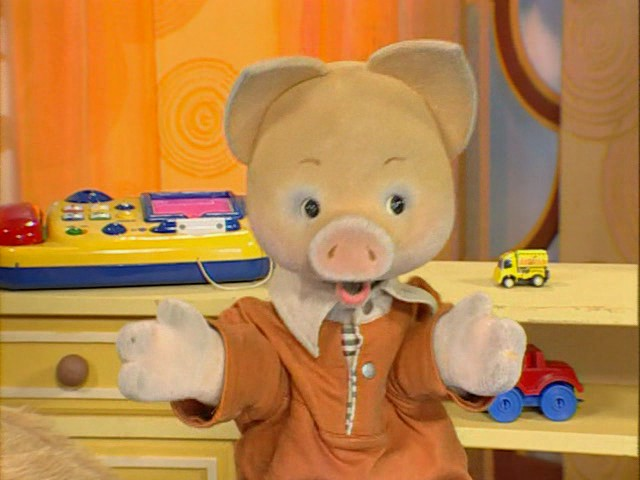
\includegraphics[height=5cm]{khrusha.jpg}

С поросячьим приветом, Хрюша.

\end{document}
